\subsubsection{Guardian API}
\label{sec:guardian-api}

As our source of global news we have chosen a British newspaper \textit{The Guardian}. Its open platform provides access to over 1.9 billion pieces of content while its \textit{Explore} tool makes it easy to search through the data. We encountered no problems requesting a developer API-key, nor were there any difficulties accessing the data. 

\textit{The Guardian} allows to extract up to 200 articles at a time, however either there is no upper limit on the number of requests one can send using one API-key or the limit is above the scope of our project.

Furthermore, one could also add such filters as "from-date", "to-date", "page size", "order-by" etc. to customise the search. We have used the date-related filters to exclude the content pieces before 2000 and after 2016 as well as increased the "page size" to the maximum of 200 items. 

Having applied the above mentioned filters, we have proceeded with extracting meta-data about ca. 40000 articles with the keyword "terror". Although OpenRefine is an easy tool to clean unsorted meta data, it proved to be inefficient in accessing over 200 URLs of data. Therefore we opted for writing scripts in Python, which would allow us to iterate over all articles without manually specifying the URL of every page. 

The script for extracting meta data from \textit{The Guardian} is similar to the one for \textit{Die Zeit}. The parameters and the keywords were adjusted, the number of items per page was set as well as only meta data was collected, without accessing individual articles. Unfortunately, the articles did not contain information on the location associated with the content piece, neither did they contain tags. 

The results of running the Python script were written into a .csv file and visualised with plot.ly.

\begin{figure}[h]
  \centering
  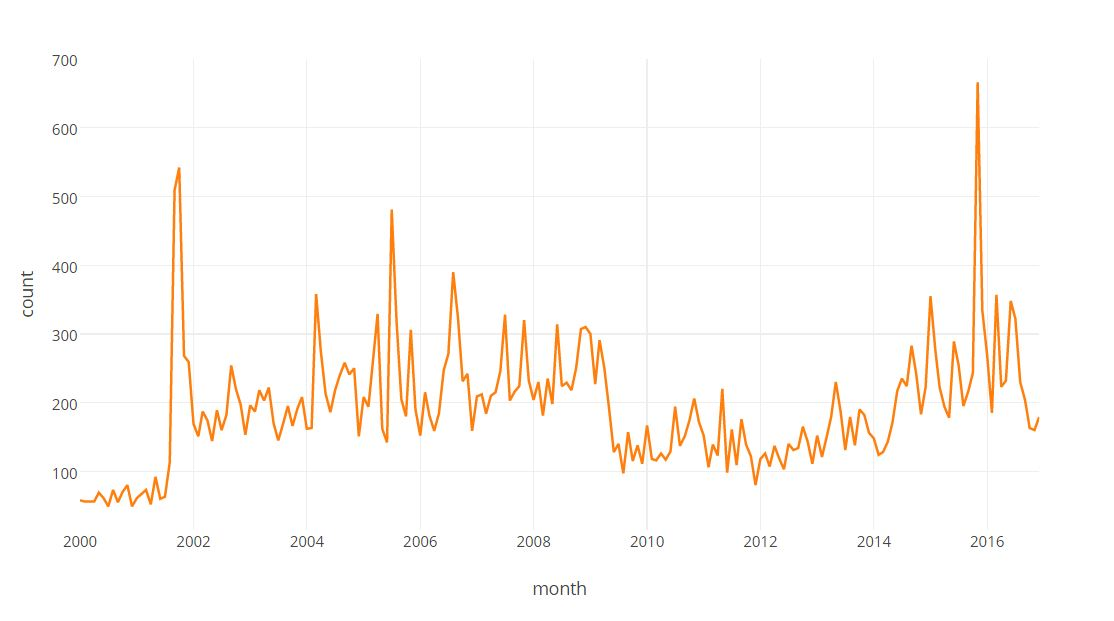
\includegraphics[width=0.7\textwidth]{images/guardian/graph_guardian_articles}
  \caption{Absolute Number of Articles with a keyword "terror" on theguardian.com between 2000-2016}
  \label{fig:guardian_total_number_of_articles}
\end{figure}


